\section{Trabalhos Relacionados} % Seções são adicionadas para organizar sua apresentação em blocos discretos, todas as seções e subseções são automaticamente exibidas no índice como uma visão geral da apresentação, mas NÃO são exibidas como slides separados.

%----------------------------------------------------------------------------------------
\begin{frame}
    \frametitle{Timeline}
    \begin{figure}
        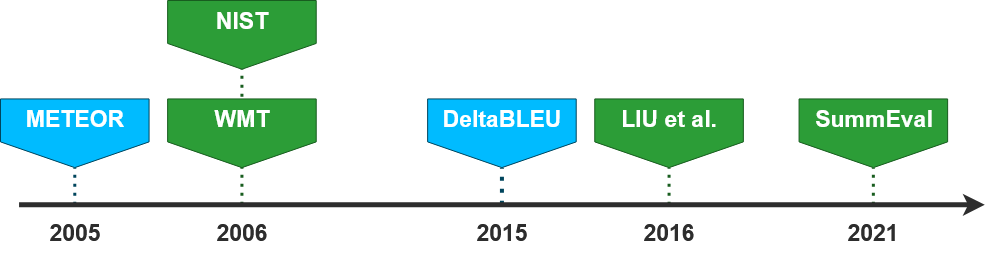
\includegraphics[width=0.9\textwidth]{TCC-timeline-trabalhos.png}
    \end{figure}
\end{frame}

%----------------------------------------------------------------------------------------
\begin{frame}
    \frametitle{SummEval}
    \only<1>{
        Um conjunto de recursos para pequisa de avaliação.
    }
    \only<2-3>{
        \begin{itemize}[<+(1)->]
            \item Sumários gerados no dataset CNN/DailyMail.
            \item Anotações humanas coletadas.
        \end{itemize}
    }
    \only<4->{
        \frametitle{Limitações do SummEval}
        \begin{itemize}[<+(4)->]
            \item Trabalha apenas com Sumarização.
            \item Focado somente na língua inglesa.
        \end{itemize}
    }
\end{frame}

%----------------------------------------------------------------------------------------
\begin{frame}
    \frametitle{Objetivo}
    \only<1>{
        Mensurar a correlação entre diferentes métricas de avaliação automatizadas e 
	    a forma de avaliação humana no âmbito de open-ended tasks.
    }
	\only<2>{
        Mensurar a correlação entre diferentes métricas de avaliação automatizadas e 
	    a forma de avaliação humana no âmbito de open-ended tasks \textbf{em português}.
    }
\end{frame}